%%%%%%%%%%%%%%%%%%%%%%%%%%%%%%%%%%%%%%%%%%%%%%%%%%%%%%%%%%%%%%%%%%%%%%
% Lớp 10 | Mệnh đề. Tập hợp | Các phép toán tập hợp
% Dạng 0D1?3-5: Toán thực tế  ứng dụng của tập hợp
% Số câu: 44  (sinh tự động bởi tach_cau.py; từ nay thầy sửa trực tiếp file này)
%%%%%%%%%%%%%%%%%%%%%%%%%%%%%%%%%%%%%%%%%%%%%%%%%%%%%%%%%%%%%%%%%%%%%%

%%%%%%%%%%%%%%%% TRẮC NGHIỆM 4 PHƯƠNG ÁN %%%%%%%%%%%%%%%%

% nguồn: MaHoaNH_TracNghiem_Lop10
\begin{ex}%[0D1N3-5]%[ma:4db901c1]
	Ký hiệu $H$ là tập hợp các học sinh của lớp $10 \mathrm{A}$. $T$ là tập hợp các học  sinh nam, $G$ là tập hợp các học sinh nữ của lớp $10 \mathrm{A}$. Khẳng định nào sau đây \textbf{sai}?
	\choice 
		{$T  \cup G=H$}
		 {$T \cap G=\varnothing$}
		 {$H \setminus T=G$}
		{\True $G \setminus  T=\varnothing$}
	\loigiai{ 
		Vì  $G \setminus T=G$.
	 }
\end{ex}

% nguồn: MaHoaNH_TracNghiem_Lop10
\begin{ex}%[0D1H3-5]%[ma:6762bf89]
	Trong kì thi học sinh giỏi cấp trường, lớp 10A có $17$ bạn được  xếp công nhận học sinh giỏi Văn, $25$ bạn học sinh giỏi Toán. Tìm số học sinh giỏi cả Văn và Toán biết lớp 10A có $45$ học sinh và có $13$ học sinh không đạt học sinh giỏi.
	 \choice
		{\True $10$} 
		{$32$} 
		{$30$} 
		 {$15$}
	\loigiai{Gọi  $A$ là tập hợp các học sinh giỏi Văn, $B$ là tập hợp các học sinh giỏi Toán.\\
		Theo đề ta có  $n(A)=17$, $n(B)=20$.\\
		Số  học sinh giỏi Văn hoặc Toán là $n(A\cup B)=45-13=32$.\\
		Khi đó số bạn giỏi cả Văn  và Toán là $$n(A\cap B)=n(A)+n(B)-n(A\cup B)=17+25-32=10.$$
	 }
\end{ex}

% nguồn: MaHoaNH_TracNghiem_Lop10
\begin{ex}%[0D1H3-5]%[ma:19658d64]
	Một lớp có $30$ học sinh, trong đó mỗi học sinh giỏi ít nhất một trong  hai môn Văn hoặc Hóa, biết rằng có $15$ bạn học giỏi môn Hóa, $20$ bạn học giỏi môn Văn. Hỏi lớp đó có bao nhiêu học sinh giỏi cả hai môn?
	\choice 
		 {$25$}
		 {$20$}
		{$10$} 
		 {\True $5$}
	\loigiai{ 
		 Gọi $A$ là tập hợp các học sinh giỏi Hóa, $B$ là tập hợp các học sinh giỏi Văn.\\
		Theo đề ta có $n(A)=15$, $n(B)=20$, $n(A\cup B)=30$.\\ 
		Khi đó số bạn giỏi cả hai môn là $$n(A\cap B)=n(A)+n(B)-n(A\cup B)=15+20-30=5.$$ 
	} 
\end{ex}

% nguồn: MaHoaNH_TracNghiem_Lop10
\begin{ex}%[0D1H3-5]%[ma:438d4fce]
	Lớp 10A có $15$ bạn được xếp loại học lực Giỏi, $20$ bạn được xếp loại hạnh kiểm Tốt, trong đó có $10$ bạn vừa được học lực Giỏi vừa được hạnh kiểm Tốt. Khi đó lớp 10A có bao nhiêu bạn được xếp loại học lực Giỏi hoặc hạnh kiểm  Tốt?
	\choice 
		 {\True $25$}
		{$20$} 
		 {$35$}
		{$40$} 
	 \loigiai{
		Gọi $A$ là tập hợp các bạn được xếp loại học lực Giỏi, $B$ là tập hợp các  bạn được xếp loại hạnh kiểm Tốt.\\
		Theo đề ta có  $n(A)=15$, $n(B)=20$, $n(A\cap B)=10$.\\
		Khi đó số bạn được xếp  loại học lực Giỏi hoặc hạnh kiểm Tốt là $$n(A\cup B)=n(A)+n(B)-n(A\cap B)=15+20-10=25.$$
	 }
\end{ex}

% nguồn: MaHoaNH_TracNghiem_Lop10
\begin{ex}%[0D1H3-5]%[ma:1f15fdfa]
	Trong số $45$ học sinh của lớp 10A có $15$ bạn được xếp loại học lực Giỏi, $20$ bạn được xếp loại hạnh kiểm Tốt, trong đó có $10$ bạn vừa được học lực Giỏi vừa được hạnh kiểm Tốt. Khi đó lớp 10A  có bao nhiêu bạn chưa được xếp loại học lực Giỏi và chưa có hạnh kiểm Tốt.
	\choice 
		{$25$} 
		{\True  $20$}
		{$35$} 
		 {$40$}
	\loigiai{ 
		Gọi $A$ là tập hợp các bạn được xếp loại học lực Giỏi, $B$ là tập hợp các bạn được xếp loại hạnh kiểm  Tốt.\\
		Theo đề  ta có $n(A)=15$, $n(B)=20$, $n(A\cap B)=10$.\\
		Khi đó số bạn được xếp loại học lực Giỏi hoặc hạnh kiểm Tốt  là $$n(A\cup B)=n(A)+n(B)-n(A\cap B)=15+20-10=25.$$
		 Số bạn chưa được xếp loại học lực Giỏi và chưa có hạnh kiểm Tốt là $45-25=20$.
	 }
\end{ex}

% nguồn: MaHoaNH_TracNghiem_Lop10
\begin{ex}%[0D1H3-5]%[ma:5330c42e]
	Mỗi học sinh  lớp $10$B đều chơi bóng đá hoặc bóng chuyền. Biết rằng có $25$ bạn chơi bóng đá, $20$ bạn chơi bóng chuyền và $10$ bạn chơi cả hai môn. Số học sinh lớp $10$B là
	 \choice
		 {$20$}
		{$25$} 
		 {$30$}
		{\True  $35$}
	 \loigiai{
	Gọi $X$ là tập hợp các học sinh của lớp $10$B; $A$ là tập hợp các  học sinh chơi bóng đá và $B$ là tập hợp các học sinh chơi bóng chuyền.\\
	Theo giả thiết $n(A)=25$, $n(B)=20$, $n(A\cap  B)=10$. \\
	Do mỗi em học sinh đều chơi ít nhất một trong hai môn nên số học sinh của lớp $10B$ là 
	$$n(A\cup B) = n(A) +  n(B) - n(A\cap B) = 25+20-10 = 35.$$
	} 
\end{ex}

% nguồn: MaHoaNH_TracNghiem_Lop10
\begin{ex}%[0D1H3-5]%[ma:145bf903]
	Lớp $10$A có $40$ học sinh trong đó có $10$ bài học sinh giỏi Toán, $15$ bạn học sinh giỏi Lý và $22$ bạn không giỏi môn học nào trong hai môn Toán, Lý. Số học sinh lớp $10A$ vừa giỏi Toán vừa giỏi Lý là 
	 \choice
		 {\True $7$}
		 {$25$}
		{$10$} 
		 {$18$}
	 \loigiai{
	Gọi $X$ là tập hợp các học sinh của lớp  $10$A; $A$ là tập hợp các học sinh giỏi Toán và $B$ là tập hợp các học sinh giỏi Lý.\\
	Theo giả thiết $n(A)=10$,  $n(B)=15$, $n(X)=40$.\\
	Do có $22$ học sinh không giỏi môn nào nên số học sinh giỏi  ít nhất một trong hai môn là
	 $$n(A\cup B) = 40 - 22 = 18.$$
	Suy  ra số học sinh của lớp $10$A giỏi cả hai môn là
	$$n(A\cap B) = n(A) + n(B) - n(A\cup B) = 10+15-18 = 7.$$ 
	} 
\end{ex}

% nguồn: MaHoaNH_TracNghiem_Lop10
\begin{ex}%[0D1H3-5]%[ma:41c794e6]
	Một lớp có $45$ học sinh. Mỗi em đều đăng ký chơi ít nhất một trong hai môn: bóng đá và bóng chuyền. Có $35$ em đăng ký môn bóng đá, $15$ em đăng ký môn bóng chuyền.  Số em học sinh đăng ký chơi cả hai môn là
	 \choice
		{$10$} 
		 {$30$}
		{\True  $5$}
		{$25$} 
	\loigiai{ 
	Gọi $X$ là tập hợp các học sinh của lớp; $A$ là tập hợp các học sinh đăng ký chơi bóng đá và $B$  là tập hợp các học sinh đăng ký chơi bóng chuyền.\\
	Theo  giả thiết $n(A)=10$, $n(B)=15$, $n(X)=40$. \\
	Do mỗi em học sinh đều đăng ký chơi ít  nhất một trong hai môn nên
	$$n(A\cup B) = n(X) = 45.$$ 
	 Suy ra số học sinh của lớp đăng ký cả hai môn là
	$$n(AB) = n(A) + n(B) - n(A\cup  B) = 35+15-45 = 5.$$
	} 
\end{ex}

% nguồn: MaHoaNH_TracNghiem_Lop10
\begin{ex}%[0D1H3-5]%[ma:f8c5997e]
	 Một lớp học có $25$ học sinh chơi bóng đá, $23$ học sinh chơi bóng bàn, $14$ học sinh chơi cả bóng đá và bóng bàn và $6$ học sinh không chơi môn nào. Số học sinh chỉ chơi $1$ môn thể thao là
	\choice 
		 {$48$}
		{\True $20$} 
		 {$34$}
		{$28$} 
	\loigiai{ 
		Gọi 
		\begin{itemize}
			\item $A$ là tập hợp các học sinh chơi  bóng đá,
			\item $B$ là tập hợp các học sinh chơi bóng bàn, 
			\item $C$ là tập hợp các  học sinh không chơi môn nào.
		\end{itemize}
		Khi đó số  học sinh chỉ chơi $1$ môn thể thao là
		 $$n(A)+n(B)-2n(A\cap B)=25+23-2\cdot 14=20.$$
	 }
\end{ex}

% nguồn: MaHoaNH_TracNghiem_Lop10
\begin{ex}%[0D1H3-5]%[ma:704299db]
	Một lớp học có $25$ học sinh giỏi môn Toán, $23$ học sinh giỏi môn Lý, $14$ học sinh giỏi cả môn Toán và Lý và có $6$ học sinh không  giỏi môn nào cả. Hỏi lớp đó có bao nhiêu học sinh?
	 \choice
		{$54$} 
		{\True $40$} 
		 {$26$}
		 {$68$}
	\loigiai{ 
		\begin{center}
			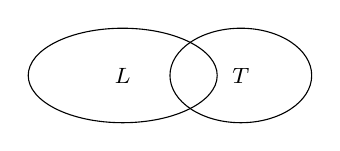
\begin{tikzpicture}[scale=.6,font=\footnotesize,line join=round,line cap=round,>=stealth]
					\draw  (3,0) arc (0:360:2 cm and 1 cm);
					\draw  (5,0) arc (0:360:1.5 cm and 1 cm);
					 \draw (1,0) node{$L$};
					 \draw (3.5,0) node{$T$};
				\end{tikzpicture}
		\end{center}
		Gọi $T$, $L$  lần lượt là tập hợp các học sinh giỏi Toán và các học sinh giỏi Lý.\\
		 Ta có\\
		$|T|$:  là số học sinh giỏi Toán\\
		$|L|$: là số học  sinh giỏi Lý\\
		$|T\cap L|$: là số học sinh giỏi cả hai môn  Toán và Lý\\
		Khi đó số học sinh  của lớp là $|T\cup L|+6$.\\
		 Mà $|T\cup L|=|T|+|L|-|T\cap L|=25+23-14=34$.\\
		Vậy số học  sinh của lớp là $34+6=40$.
	 }
\end{ex}

% nguồn: MaHoaNH_TracNghiem_Lop10
\begin{ex}%[0D1H3-5]%[ma:415ca498]
	Trong kì thi học sinh  giỏi cấp trường lớp 11B1 có $15$ học sinh giỏi Văn, $22$ học sinh giỏi Toán. Tìm số học sinh giỏi cả Văn và Toán biết lớp 11B1 có $40$ học sinh và có $14$ học sinh không đạt học sinh giỏi.
	 \choice
		{$4$} 
		 {$7$}
		 {\True $11$}
		{$20$} 
	 \loigiai{
		\begin{center}
			\begin{tikzpicture}[scale=1,font=\footnotesize,line join=round,line cap=round,>=stealth]
					\def\miena{(0,0) ellipse (1.8  and 1.6)};
					\def\mienb{(2,0) ellipse (1.6 and  1.4)};
					\begin{scope}
						 \clip\miena;
						\fill[pattern=north  west lines]\mienb;
					\end{scope}
					\draw\miena  \mienb;
					 \draw (-0.6,1.6) node[above]{$22$(Toán)}
						(2.6,1.6)  node[above]{$15$(Văn)};
				\end{tikzpicture}
		\end{center}
		{\it Cách 1.}\\ 
		Số học sinh học giỏi  ít nhất một trong hai môn Toán và Văn là $40-14=26$.\\
		Số  học sinh chỉ giỏi Toán mà không giỏi Văn (phần Toán sau khi bỏ đi phần giao)
		là  $$26-15=11.$$
		Vậy số  học sinh giỏi cả hai môn Toán và Văn (phần giao nhau) là $22-11=11$.\\
		 {\it Cách 2.}\\
		Số học sinh học giỏi ít nhất một trong hai môn  Toán và Văn là $40-14=26$.\\
		Số học  sinh giỏi cả hai môn Toán và Văn là $22+15-26=11$.
	} 
\end{ex}

% nguồn: MaHoaNH_TracNghiem_Lop10
\begin{ex}%[0D1H3-5]%[ma:7b3217d0]
	Một lớp học có $25$ học sinh giỏi môn Toán, $23$ học sinh giỏi môn Lý,  $14$ học sinh giỏi cả môn Toán và Lý và có 6học sinh không giỏi môn nào cả. Hỏi lớp đó có bao nhiêu học sinh?
	\choice 
		{$54$} 
		 {\True $40$}
		 {$26$}
		 {$68$}
	 \loigiai{
	\immini{Gọi $T$, $L$ lần lượt là tập hợp các học  sinh giỏi Toán và các học sinh giỏi Lý.
		 Ta có
		\begin{itemize}
			\item 
			$n(T)$ là  số học sinh giỏi Toán,
			\item $n(L)$ là số học  sinh giỏi Lý,
			\item $n(T\cap L)$ là số học sinh giỏi cả  hai môn Toán và Lý.
		\end{itemize}
		}{\begin{tikzpicture}[scale=1,font=\footnotesize,line join=round,line cap=round,>=stealth]
		\def\miena{(0,0) ellipse (1.8 and  1.6)};
		\def\mienb{(2,0) ellipse (1.6 and  1.4)};
		\begin{scope}
			\clip\miena; 
			 \fill[pattern=crosshatch dots]\mienb;
		\end{scope}
		 \draw\miena \mienb;
		\draw  (-0.6,1.6) node[above]{$T$}
			 (2.6,1.6) node[above]{$L$}
			(1,0) node[fill=white,inner sep=2pt]{$T\cap  L$};
	\end{tikzpicture}
		}\noindent 
		Khi đó số học sinh của lớp  là $n(T\cup L)+6$ mà $$n(T\cup L)=n(T)+n(L)-n(T\cap L)=25+23-14=34.$$
		Vậy số học  sinh của lớp là $34+6=40$.
	} 
\end{ex}

% nguồn: MaHoaNH_TracNghiem_Lop10
\begin{ex}%[0D1H3-5]%[ma:fc977dab]
	Mỗi học sinh  của lớp $10A_1$ đều học giỏi môn Toán hoặc môn Hóa, biết rằng có $30$ học sinh giỏi Toán, $35$ học sinh giỏi Hóa, và $20$ em học giỏi cả hai môn. Hỏi lớp $10A_1$ có bao nhiêu học sinh?
	\choice 
		 {$40$}
		{\True $45$} 
		 {$50$}
		{$55$} 
	\loigiai{ 
		\begin{center}
			\begin{tikzpicture}[scale=1,font=\footnotesize,line join=round,line cap=round,>=stealth]
					\def\miena{(0,0) ellipse (1.6  and 1.4)};
					\def\mienb{(2,0) ellipse (1.8 and 1.6)}; 
					\begin{scope}
						 \clip\miena;
						 \fill[pattern=crosshatch dots]\mienb;
					\end{scope}
					\draw\miena \mienb; 
					 \draw (-0.6,1.6) node[above]{$30$(Toán)}
						(2.6,1.6)  node[above]{$35$(Hóa)}
						(1,0) node[fill=white,inner  sep=2pt]{$20$};
				\end{tikzpicture}
		\end{center}
		 {\it Cách 1.}\\
		Dựa vào  biểu đồ ven ta có
		\begin{itemize}
			\item Số học sinh chỉ giỏi môn Toán là $30-20=10$. 
			\item Số học sinh chỉ giỏi  môn Hóa là $35-20=15$.
		\end{itemize}
		Do đó số học $\sinh$ lớp $10A_1$ là  $10+20+15=45$.\\
		{\it Cách  2.}\\
		Sĩ số học sinh lớp  $10A_1$ là $30+35-20=45$.
	 }
\end{ex}

% nguồn: MaHoaNH_TracNghiem_Lop10
\begin{ex}%[0D1H3-5]%[ma:1d662c9d]
	Lớp 10A có $45$ học sinh trong đó có $25$ em học giỏi môn Toán, $23$ em học giỏi  môn Lý, $20$ em học giỏi môn Hóa, $11$ em học giỏi cả môn Toán và môn Lý, $8$ em học giỏi cả môn Lý và môn Hóa, $9$ em học giỏi cả môn Toán và môn Học. Hỏi lớp $10$ A có bao nhiêu bạn học giỏi cả ba môn Toán, Lý, Hóa, biết rằng mỗi học sinh trong lớp học giỏi ít nhất một trong $3$ môn Toán, Lý, Hóa?
	\choice 
		{$3$} 
		 {$4$}
		 {\True $5$}
		{$6$} 
	 \loigiai{
		\begin{center}
			\begin{tikzpicture}[scale=.8,font=\footnotesize,line join=round,line cap=round,>=stealth]
					\coordinate  (A) at (0,0);
					 \coordinate (B) at (2,0);
					\coordinate  (C) at (1,-1.5);
					\begin{scope}
						 \clip (C) circle (1.5);
						 \clip (A) circle (1.5);
						\fill[pattern=north west lines]  (B) circle (1.5);
					\end{scope}
					\draw (A)  circle (1.5);
					\draw (B)  circle (1.5);
					\draw (C) circle  (1.5);
					 \path
						 (A)++(90:.6) node[fill=white,above]{$L$}
						(B)++(90:.6)  node[fill=white,above]{$T$}
						(C)++(-90:1)  node[fill=white,above]{$H$};
				\end{tikzpicture}
		\end{center}
		Gọi $T$, $L$, $H$ lần lượt là tập hợp các học sinh giỏi môn Toán,  Lý, Hóa.\\
		Khi đó 
		\begin{eqnarray*}
			|T \cup L \cup H|&=&|T|+|L|+|H|-|T \cap L|-|L \cap H|-|H \cap T|+|T \cap L  \cap H| \\
			 45&=&25+23+20-11-8-9+|T \cap L \cap H|\\
			|T  \cap L \cap H|&=&5
		\end{eqnarray*}
		Vậy có $5$ học  sinh giỏi cả $3$ môn.
	 }
\end{ex}

% nguồn: MaHoaNH_TracNghiem_Lop10
\begin{ex}%[0D1V3-5]%[ma:feea80e0]
	Lớp 10A có $7$ học sinh giỏi Toán, $5$ học sinh giỏi Lý, $6$ học sinh giỏi Hóa, $3$ học sinh giỏi cả Toán và Lý, $4$ học sinh giỏi cả Toán và Hóa, $2$ học sinh giỏi cả  Lý và Hóa, $1$ học sinh giỏi cả ba môn Toán, Lý, Hóa. Số học giỏi ít nhất một môn (Toán, Lý, Hóa) của lớp 10A là
	 \choice
		 {$18$}
		{\True  $10$}
		{$9$} 
		 {$28$}
	 \loigiai{
		 Gọi
		\begin{itemize}
			\item $A$ là tập hợp các học  sinh giỏi Toán;
			\item $B$ là tập hợp các  học sinh giỏi Lý;
			\item $C$ là tập hợp các học  sinh giỏi Hóa.
		\end{itemize}
		Học sinh giỏi ít nhất một môn  là tập hợp $A\cup B\cup C$.\\
		 Ta có
		\begin{align*}
			n(A\cup B\cup C)&=n(A)+n(B)+n(C)-n(A\cap  B)-n(A\cap C)-n(B\cap C)+n(A\cap B\cap C)\\
			 &=7+5+6-3-4-2+1=10.
		\end{align*}
	} 
\end{ex}

% nguồn: MaHoaNH_TracNghiem_Lop10
\begin{ex}%[0D1V3-5]%[ma:122f3f0e]
	Lớp 10A có $45$ học sinh trong đó có $25$ em học giỏi môn Toán, $23$ em học giỏi môn Lý, $20$ em học giỏi môn Hóa, $11$ em học giỏi cả môn Toán và môn Lý, $8$ em học giỏi  cả môn Lý và môn Hóa, $9$ em học giỏi cả môn Toán và môn Hóa). Hỏi lớp 10A có bao nhiêu bạn học giỏi cả ba môn Toán, Lý, Hóa, biết rằng mỗi học sinh trong lớp học giỏi ít nhất một trong $3$ môn Toán, Lý, Hóa?
	\choice 
		{$3$} 
		 {$4$}
		{\True $5$} 
		 {$6$}
	\loigiai{ 
		Gọi $T$, $L$, $H$ lần lượt là tập hợp  các học sinh giỏi môn Toán, Lý, Hóa.
		\begin{center}
			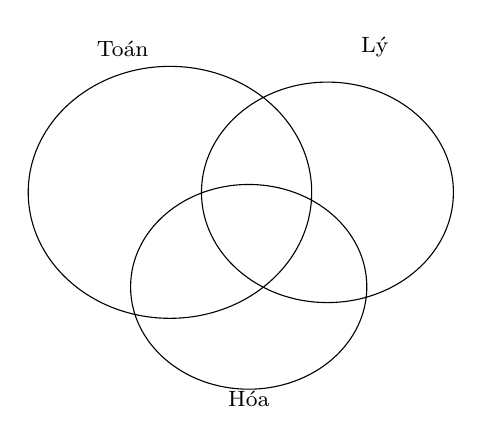
\begin{tikzpicture}[scale=1,font=\footnotesize,line join=round,line cap=round,>=stealth]
					\def\miena{(0,0) ellipse  (1.8 and 1.6)};
					\def\mienb{(2,0)  ellipse (1.6 and 1.4)};
					\def\mienc{(1,-1.2)  ellipse (1.5 and 1.3)};
					\draw\miena \mienb  \mienc;
					\draw  (-0.6,1.6) node[above]{Toán}
						(2.6,1.6) node[above]{Lý} 
						(1,-2.4)  node[below]{Hóa};
				\end{tikzpicture}
		\end{center}
		Ta có công thức 
		\begin{eqnarray*}
			&&n(T\cup L\cup H)=n(T)+n(L)+n(H)-n(T\cap L)-n(L\cap H)-n(H\cap T)+n(T\cap L\cap  H)\\
			 &\Leftrightarrow & 45=25+23+20-11-8-9+n(T\cap L\cap H)\\
			&\Leftrightarrow & n(T\cap L\cap H)=5. 
		\end{eqnarray*}
		Vậy có $5$  học sinh giỏi cả $3$ môn.
	} 
\end{ex}

% nguồn: MaHoaNH_TracNghiem_Lop10
\begin{ex}%[0D1V3-5]%[ma:edb9d33c]
	Hội khỏe Phù Đổng của trường Trần Phú, lớp 10A có $45$ học sinh, trong đó có $25$ học sinh thi  điền kinh, $20$ học sinh thi nhảy xa, $15$ học sinh thi nhảy cao, $7$ em không tham gia môn nào, $5$ em tham gia cả $3$ môn. Hỏi số em tham gia chỉ một môn trong ba môn trên là bao nhiêu?
	\choice 
		 {$20$}
		{$45$} 
		 {$38$}
		 {\True $21$}
	 \loigiai{
		\begin{center}
			\begin{tikzpicture}[scale=1,font=\footnotesize,line join=round,line cap=round,>=stealth]
					\draw (0,0) ellipse (2  and 1.8)
						(2,0)  ellipse (2 and 1.8)
						(1,-1.8) ellipse (1.6  and 1.4);
					\draw (-0.8,1.8)  node[above]{$20$(Điền kinh)}
						(2.8,1.8) node[above]{$20$(Nhảy xa)} 
						(1,-3.2) node[below]{$15$(Nhảy  cao)}
						(1,-1)  node[]{$5$}
						 (1,0.3) node[]{$x$}
						(2.6,0) node[]{$b$} 
						(-0.6,0) node[]{$a$} 
						(2,-1.3)  node[]{$y$}
						 (0,-1.3) node[]{$z$}
						 (1,-2.2) node[]{$c$};
				\end{tikzpicture}
		\end{center}
		Gọi 
		\begin{itemize}
			\item $a$, $b$, $c$ theo thứ tự là số học sinh chỉ thi môn điền kinh,  nhảy xa, nhảy cao,
			\item $x$ là số học sinh chỉ thi hai môn điền kinh và nhảy  xa,
			\item $y$ là số học sinh chỉ thi hai môn nhảy xa và nhảy cao, 
			 \item $z$ là số học sinh chỉ thi hai môn điền kinh và nhảy cao.
		\end{itemize}
		Số em thi ít nhất  một môn là $45-7=38$.\\
		Dựa vào biểu đồ ven ta có hệ phương trình  sau $$\heva{&a+x+z+5=25&&(1)\\
		&b+x+y+5=20&&(2)\\ 
		 &c+y+z+5=15&&(3)\\
		 &x+y+z+a+b+c+5=38.&&(4)}$$
		Cộng vế với vế của $(1)$, $(2)$, $(3)$ ta  có $$a+b+c+2(x+y+z)+15=60.\quad (5)$$
		Từ $(4)$, $(5)$  ta có $$a+b+c+2(38-5-a-b-c)+15=60\Leftrightarrow a+b+c=21.$$
		Vậy  có $21$ học sinh chỉ thi một trong ba nội dung trên.
	 }
\end{ex}


%%%%%%%%%%%%%%%% ĐÚNG/SAI %%%%%%%%%%%%%%%%

% nguồn: MaHoaNH_DungSai_Lop10
\begin{ex}%[0D1H3-5]%[ma:bdb7af9e]
	Một lớp có $40$ học sinh, biết rằng ai cũng đăng kí thi ít nhất một trong hai môn là cờ vua và cờ tướng. Có $17$ em đăng kí  môn cờ vua, $28$ em đăng kí môn cờ tướng.
	 \choiceTF
		{Có $28$ học sinh chỉ đăng kí môn cờ  tướng}
		{Số học sinh đăng kí môn cờ vua là $17$ học  sinh}
		{\True Số  học sinh đăng kí môn cờ tướng là $28$ học sinh}
		{\True Có tất cả $5$ học sinh đăng kí cả hai môn  cờ}
	\loigiai{ 
		Gọi \begin{itemize}
		 \item $x$ là số học sinh chỉ đăng kí môn cờ vua,
		\item $y$ là số học sinh chỉ đăng kí môn cờ tướng, 
		\item $z$ là số học sinh tham gia  cả hai môn này.
	\end{itemize}
	Số học sinh đăng kí môn cờ vua là $17$ học  sinh nên $x+z=17\Leftrightarrow x=17-z$.\\
	Số  học sinh đăng kí môn cờ tướng là $28$ học sinh nên $y+z=28\Leftrightarrow y=28-z$.\\
	Vì tổng số học sinh  lớp đó là $40$ học sinh nên ta có $$x+y+z=40\Leftrightarrow 17-z+28-z+z=40\Leftrightarrow z=5.$$
	Vậy  số học sinh đăng kí cả hai môn cờ là $5$ học sinh.
	\begin{itemchoice}
		\itemch 
		Có $28-5=23$ học sinh chỉ đăng kí môn cờ tướng. 
		\itemch Số học sinh  chỉ đăng kí môn cờ vua là $17-5=12$ học sinh.
		\itemch Số học sinh đăng kí môn cờ tướng là $28$ học  sinh.
		\itemch Có tất cả $5$ học sinh đăng kí cả hai  môn cờ.
	\end{itemchoice}
 }
\end{ex}

% nguồn: MaHoaNH_DungSai_Lop10
\begin{ex}%[0D1V3-5]%[ma:b74da9f4]
	Lớp 10A có $35$ học sinh thi học sinh giỏi. Mỗi học sinh thi ít nhất một môn trong ba môn Toán, Lý và Hóa. Biết có $12$ học sinh chỉ thi môn Toán, có $14$ học sinh thi môn Lý, có $15$ học sinh thi môn Hóa và có $3$ học sinh chỉ thi môn Lý  và môn Hóa.
	 \choiceTF
		{Có $9$ học sinh chỉ thi môn Lý mà  không thi môn Hóa}
		{Có $23$ học sinh chỉ thi môn Hóa mà  không thi môn Lý}
		{Số học sinh chỉ thi môn Lý hoặc thi môn Hóa là $8$ học  sinh}
		{\True  Có $3$ học sinh đi thi cả ba môn Toán, Lý và Hoá}
	\loigiai{ 
		\begin{center}
			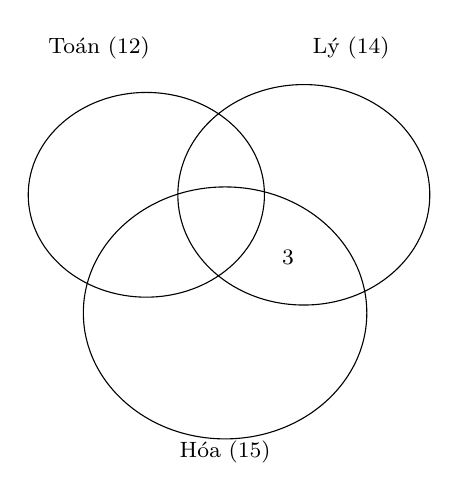
\begin{tikzpicture}[scale=1,font=\footnotesize,line join=round,line cap=round,>=stealth]
					\def\miena{(0,0) ellipse (1.5  and 1.3)};
					\def\mienb{(2,0) ellipse (1.6 and  1.4)};
					\def\mienc{(1,-1.5) ellipse (1.8 and  1.6)};
					 \draw\miena \mienb \mienc;
					\draw  (-0.6,1.6) node[above]{Toán ($12$)}
						 (2.6,1.6) node[above]{Lý ($14$)}
						(1,-3) node[below]{Hóa ($15$)} 
						 (1.8,-0.8) node[]{$3$};
				\end{tikzpicture}
		\end{center}
		Số học sinh chỉ thi môn Lý hoặc thi  môn Hóa là $35-12=23$ học sinh.\\
		Số học sinh chỉ thi môn Lý mà không thi môn  Hóa là $23-15=8$ học sinh.\\
		Số học sinh chỉ thi môn Hóa mà  không thi môn Lý là $23-14=9$ học sinh.\\
		Số học sinh thi môn Lý và môn  Hóa là $23-(8+9)=6$ học sinh.\\
		Số học sinh thi cả ba  môn là $6-3=3$ học sinh.
		\begin{itemchoice}
			\itemch Có  $8$ học sinh chỉ thi môn Lý mà không thi môn Hóa.
			 \itemch Có $9$ học sinh chỉ thi môn Hóa mà không thi môn Lý.
			\itemch Số học sinh chỉ thi môn Lý hoặc thi môn Hóa là $23$ học  sinh.
			\itemch Có $3$ học  sinh đi thi cả ba môn Toán, Lý và Hoá.
		\end{itemchoice}
	} 
\end{ex}

% nguồn: MaHoaNH_DungSai_Lop10
\begin{ex}%[0D1V3-5]%[ma:7293d844]
	Các em học sinh lớp $10A$ làm bài thi khảo sát học sinh giỏi môn Toán. Đề thi có $3$  câu. Sau khi chấm bài, giáo viên tổng kết được như sau: Có $6$ học sinh làm được câu $1$, có $5$ học sinh làm được câu $2$, có $4$ học sinh làm được câu $3$. Có $2$ học sinh làm được câu $1$ và câu $2$, có $2$ học sinh làm được câu $1$ và câu $3$, có $1$ học sinh làm được câu $2$ và câu $3$ và chỉ có $1$ học sinh làm được cả $3$ câu. Xét tính đúng sai của các khẳng định sau:
	\choiceTF 
		{Có duy nhất một học sinh chỉ làm được câu $1$} 
		{\True Không có học sinh nào chỉ làm được câu $2$  và câu $3$}
		{\True Có $2$ học  sinh chỉ làm được câu $3$}
		{\True Có tất cả $8$ học sinh chỉ làm được đúng  một câu}
	\loigiai{ 
		\begin{center}
			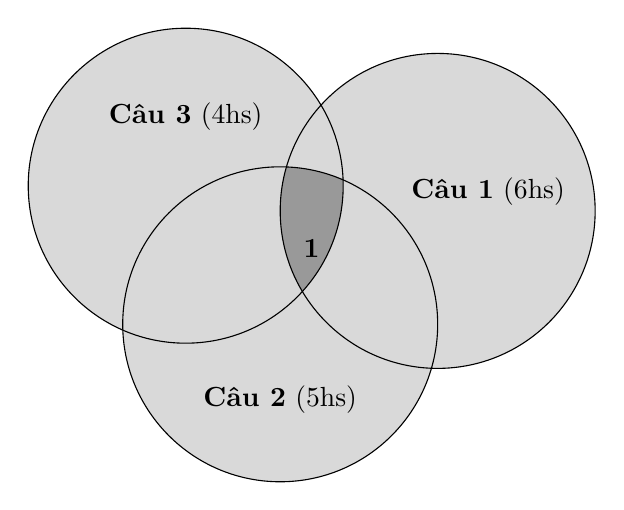
\begin{tikzpicture}[scale=0.8]
					\begin{scope}
						\fill[gray!30] (0,0) circle (2.5); 
						\fill[gray!30] (2.5,1.8) circle (2.5); 
						\fill[gray!30] (-1.5,2.2) circle  (2.5);
					\end{scope}
					\begin{scope}
						\clip (0,0) circle (2.5); 
						 \clip (2.5,1.8) circle (2.5);
						\fill[gray!80] (-1.5,2.2) circle  (2.5);
					\end{scope}
					 \draw (0,0) circle (2.5);
					\draw (2.5,1.8) circle (2.5); 
					\draw  (-1.5,2.2) circle (2.5);
					\node at (0.5,1.2)  {\textbf{1}};
					\node at (3.3,2.1)  {\textbf{Câu 1}
						($6$hs)}; 
					 \node at (0,-1.2) {\textbf{Câu 2}
						($5$hs)}; 
					\node at (-1.5,3.3)  {\textbf{Câu 3}
						($4$hs)}; 
				\end{tikzpicture}
		\end{center}
		Số học sinh chỉ làm  được câu $1$ và câu $2$ là $2 - 1 = 1$ học sinh.\\
		Số học sinh chỉ làm được câu $1$ và  câu $3$ là $2 - 1 = 1$ học sinh.\\
		Số học sinh chỉ làm được câu $2$ và câu $3$ là $1  - 1 = 0$ học sinh.\\
		Số học sinh chỉ làm được câu $1$ là $6 - (1 +  1 + 1) = 3$ học sinh.\\
		Số học sinh chỉ làm được câu $2$  là $5 - (1 + 1 + 0) = 3$ học sinh.\\
		 Số học sinh chỉ làm được câu $3$ là $4 - (1 + 1 + 0) = 2$ học sinh.\\
		Vậy số học sinh chỉ làm được $1$ câu là $3  + 3 + 2 = 8$ học sinh.
		\begin{itemchoice}
			\itemch \textbf{Sai}.\\  Có $3$ học sinh chỉ làm được câu $1$.
			\itemch \textbf{Đúng}.\\ Không có học sinh  nào chỉ làm được câu $2$ và câu $3$.
			\itemch \textbf{Đúng}.\\ Có $2$ học sinh chỉ  làm được câu $3$.
			\itemch \textbf{Đúng}.\\ Có tất cả $8$ học sinh chỉ làm  được đúng một câu.
		\end{itemchoice}
	 }
\end{ex}

% nguồn: MaHoaNH_DungSai_Lop10
\begin{ex}%[0D1V3-5]%[ma:6abb0ba4]
	Trong đợt quyên góp ủng hộ đồng bào bị lũ lụt năm $2\,020$, có $25$ học sinh lớp $12A$ đã tham gia ủng hộ, mỗi học sinh ủng hộ nhiều nhất $2$ tờ tiền khác nhau trong ba loại tờ tiền mệnh giá $5\, 000$ đồng, $10\, 000$ đồng và $20\, 000$ đồng. Biết rằng số học  sinh đã tham gia ủng hộ thỏa đồng thời ba kết quả sau:
	\begin{itemize}
		\item Số học sinh chỉ ủng hộ một tờ $5\, 000$ đồng bằng tổng số học sinh chỉ ủng hộ một tờ $10\, 000$ đồng và số học sinh chỉ ủng  hộ một tờ $20\, 000$ đồng.
		\item Trong số học sinh không ủng hộ tờ $5\, 000$ đồng thì số học sinh có ủng hộ tờ $10\, 000$ đồng nhiều gấp hai lần số học sinh có ủng hộ tờ $20\, 000$  đồng.
		\item Số học sinh chỉ ủng hộ một tờ $5\, 000$ đồng nhiều hơn số  học sinh ủng hộ tờ $5\, 000$ đồng và một tờ khác là $1$ học sinh.
	\end{itemize}
	Xét tính đúng  sai của các khẳng định sau:
	 \choiceTF
		{\True Có $2$ học sinh ủng hộ  một tờ $10\, 000$ đồng và một tờ $20\, 000$ đồng}
		{\True Có $8$ học sinh chỉ ủng  hộ một tờ $5\, 000$ đồng}
		{Nếu gọi số học sinh  ủng hộ một tờ $5\, 000$ đồng và một tờ $10\, 000$ đồng là $a$ và số học sinh ủng hộ một tờ $20\, 000$ đồng và một tờ $5\, 000$ đồng là $c$ thì $9a = c$}
		{\True Có $6$  học sinh lớp $12A$ chỉ ủng hộ một tờ $10\, 000$ đồng}
	\loigiai{ 
		\begin{center}
			\begin{tikzpicture}
					\draw[very thick] (0,0) circle (3.5cm); 
					\foreach \angle  in {0,80,120,200,240,320}{
						\draw[very thick]  (0,0) -- (\angle:3.5cm);
					} 
					\node at (30:1.8cm) {$y$}; 
					\node at (30:2.5cm) {($10\,000\text{đ}$)}; 
					\node at  (90:1.8cm) {$b$};
					\node  at (150:1.8cm) {$z$};
					\node at (150:2.5cm)  {($20\,000\text{đ}$)};
					\node at  (210:1.8cm) {$c$};
					\node at (270:1.8cm)  {$x$};
					\node at (270:2.5cm) {($5\,000\text{đ}$)}; 
					\node at (330:1.8cm) {$a$}; 
				\end{tikzpicture}
		\end{center}
		Gọi số học sinh chỉ ủng hộ một tờ $5\, 000$, $10\,  000$, $20\, 000$ đồng lần lượt là $x$, $y$, $z$.\\
		 Số học sinh ủng hộ $5\, 000$ đồng và $10\, 000$ đồng: $a$.\\
		Số học sinh ủng hộ $10\, 000$ đồng và $20\,  000$ đồng: $b$.\\
		Số học sinh ủng hộ $20\, 000$ đồng và $5\, 000$  đồng: $c$.\\
		Ta có  hệ phương trình:
		$$\heva{&x = y +  z \quad \text{(1)} \\
		&y  + b = 2(z + b) \quad \text{(2)} \\
		&x = a + c + 1  \quad \text{(3)} \\
		&x + y +  z + a + b + c = 25. \quad \text{(4)}}$$
		Từ $(2)$: $y + b = 2z + 2b \Rightarrow y = 2z +  b$.\\
		Thế vào $(1)$: $x = y  + z = 2z + b + z = 3z + b$.\\
		Thế vào $(3)$: $3z + b = a + c + 1 \Rightarrow a + c = 3z + b -  1$.\\
		Thế vào $(4)$: $x  + y + z + a + b + c = 25$:\\
		Thay $x = 3z + b$, $y = 2z  + b$, $a + c = 3z + b - 1$ vào
		\[ 
		(3z + b) + (2z + b) + z + (3z + b -  1) + b = 25
		\Rightarrow 9z + 4b =  26.
		 \]
		Do $z$, $b$ nguyên không âm, nghiệm phù hợp nên $$z = 2, b = 2 \Rightarrow y = 6, x = 8, a  + c = 7.$$
		\begin{itemchoice}
			\itemch \textbf{Đúng}.\\ Có $2$ học sinh ủng hộ một tờ $10\, 000$ đồng và  một tờ $20\, 000$ đồng ($b = 2$).
			\itemch \textbf{Đúng}.\\ Có $8$ học sinh chỉ ủng hộ một tờ $5\, 000$ đồng ($x  = 8$).
			\itemch  \textbf{Sai}.\\ Ta có $a + c = 7 \ne 9a = c$.
			\itemch \textbf{Đúng}.\\ Có $6$ học sinh lớp $12A$ chỉ ủng hộ một tờ $10\,  000$ đồng ($y = 6$).
		\end{itemchoice}
	} 
\end{ex}


%%%%%%%%%%%%%%%% TRẢ LỜI NGẮN %%%%%%%%%%%%%%%%

% nguồn: MaHoaNH_TraLoiNgan_Lop10
\begin{bt}%[0D1H3-5]%[ma:5f15144c]
	 Lớp 10A có $45$ học sinh trong đó có $12$ bạn học sinh giỏi Văn, $ 9$ bạn học sinh giỏi Địa lí, và $30$ bạn không giỏi môn học nào trong hai môn Văn, Địa lí. Hỏi lớp $10A$ có bao nhiêu bạn học sinh giỏi cả hai môn Văn và Địa lí?
	 \shortans{6}
	\loigiai{ 
	\immini{Số  học sinh giỏi Văn hoặc giỏi Địa lí là $45 - 30=15$ (học sinh).\\
		Số học sinh giỏi cả 2 môn Văn và Địa lí là  $12+9-15=6$ (học sinh).}
		{\begin{tikzpicture}
		\draw  (-3,-1.5) rectangle (3,3);
		 \draw (-1,1) circle (1.41)
			(1,1) circle  (1);
		\draw (0,-1) node[below]{$\tiny{\text{30 học sinh không giỏi Văn và Địa}}$}; 
		\draw (-1,1.5) node[below]{$\tiny{\text{12 HS giỏi  Văn}}$};
		 \draw (1.15,1) node[below]{$\tiny{\text{9 HS giỏi Địa}}$};
		\draw (0,3.5)  node[below]{$\tiny{\text{Lớp 10A có 45 học sinh}}$};
	\end{tikzpicture}
		 }
	} 
\end{bt}

% nguồn: MaHoaNH_TraLoiNgan_Lop10
\begin{bt}%[0D1H3-5]%[ma:e2e394ab]
	Lớp $11A$ có $50$  học sinh, trong đó có $20$ học sinh tham gia cuộc thi khoa học kỹ thuật, $25$ học sinh tham gia cuộc thi toán học cấp trường và $10$ học sinh không tham gia cả hai cuộc thi này. Hỏi có bao nhiêu học sinh của lớp $11A$ tham gia đồng thời cả hai cuộc thi?
	 \shortans{5}
	 \loigiai{
		Gọi $x$ là học sinh của lớp  $11A$ tham gia đồng thời cả hai cuộc thi.\\
		 Ta có sơ đồ Ven:
		\begin{center}
			\begin{tikzpicture}[
						 set/.style={draw,ellipse,minimum height=2cm,minimum width=3.5cm},
						outerbox/.style={draw,rectangle,minimum height=3.5cm,minimum width=6.5cm}] 
					 \node[outerbox,label={[anchor=south east,yshift=-0.1cm]south east:$50$}] (box) {};
					\coordinate  (A_center) at (-1.1,0);
					\coordinate  (B_center) at (1.1,0);
					\node[set,label={[yshift=0.2cm]above:$10$}] (A) at  (A_center) {};
					\node[set,label={[yshift=0.2cm]above:$ $}] (B) at (B_center) {}; 
					\node at ($(A_center) + (-0.7,0)$) {20}; 
					 \node at ($(B_center) + (0.7,0)$) {25};
					\coordinate (intersection_center) at  (0,0);
					\node at (intersection_center) {$x$}; 
				\end{tikzpicture}
		\end{center}
		Số học sinh tham gia ít nhất một trong hai cuộc thi là $50-10=40$ (học sinh).\\ 
		Từ sơ đồ Ven  ta có số học sinh lớp $11A$ tham gia đồng thời cả hai cuộc thi là
		$$x=20+25-40=5 \text{ (học  sinh)}.$$
	 }
\end{bt}

% nguồn: MaHoaNH_TraLoiNgan_Lop10
\begin{bt}%[0D1V3-5]%[ma:9396b56a]
	Một lớp học có $25$ học sinh chơi bóng đá, $23$ học sinh chơi bóng bàn, $14$ học sinh chơi cả bóng đá và bóng bàn, $6$ học sinh không chơi môn nào.  Tìm số học sinh chỉ chơi một môn thể thao.
	\shortans{20} 
	\loigiai{ 
		Gọi $A$ là  tập hợp các học sinh chơi bóng đá, $B$ là tập hợp các học sinh chơi bóng bàn, $C$ là tập hợp các học sinh không chơi môn thể thao nào.\\
		Ta có $A$: là số học sinh chơi bóng đá; $B$: là số học sinh chơi bóng bàn; $C$: là số học sinh không  chơi môn thể thao nào.\\
		Khi đó  số học sinh chỉ chơi một môn thể thao là $25 + 23 - 2 \cdot 14 = 20$.
	} 
\end{bt}

% nguồn: MaHoaNH_TraLoiNgan_Lop10
\begin{bt}%[0D1V3-5]%[ma:942bf130]
	Có $7$ vận động viên TDTT đều được đăng kí ít nhất một môn bóng bàn, cầu lông. Kết quả có $4$ vận  động viên đăng kí bóng bàn, $5$ vận động viên đăng kí cầu lông. Hỏi có bao nhiêu vận động viên chỉ đăng kí môn cầu lông?
	\shortans{3} 
	 \loigiai{
		Gọi $A$ là tập hợp các vận động viên đăng kí bóng bàn, $B$ là tập hợp các vận động viên đăng kí cầu lông.\\ 
		 Ta có
		 \[
		n(A \cup B) = 7,\quad n(A) = 4,\quad  n(B) = 5.
		\] 
		Suy  ra
		\[ 
		n(B \setminus A) =  n(B) - n(A \cap B) = n(A \cup B) - n(A) = 7 - 4 = 3.
		 \]
		Vậy có $3$ vận  động viên chỉ đăng kí môn cầu lông.
	} 
\end{bt}

% nguồn: MaHoaNH_TraLoiNgan_Lop10
\begin{bt}%[0D1V3-5]%[ma:b0e3180a]
	Bạn A.Súa thống kê số ngày có mưa, có sương mù ở bản mình trong tháng $3$ vào một thời điểm nhất định và được kết quả như sau: $14$ ngày có mưa, $15$ ngày có sương mù, trong đó $10$ ngày có cả mưa và sương mù. Hỏi trong tháng $3$ đó có bao nhiêu ngày không có mưa và không có sương mù? 
	 \shortans{12}
	\loigiai{ 
		Gọi $A$ là tập hợp các ngày  có mưa, $B$ là tập hợp các ngày có sương mù.\\
		Ta có 
		\[ 
		n(A) = 14,\quad n(B) = 15,\quad n(A  \cap B) = 10.
		\] 
		Suy ra  số ngày có mưa hoặc có sương mù là
		 \[
		n(A \cup B) = n(A) + n(B) - n(A \cap B) = 14 +  15 - 10 = 19.
		 \]
		 Tháng $3$ có $31$ ngày nên số ngày không có mưa và không có sương mù là
		\[ 
		31 - 19 = 12 \text{ (ngày)}. 
		 \]
	} 
\end{bt}

% nguồn: MaHoaNH_TraLoiNgan_Lop10
\begin{bt}%[0D1V3-5]%[ma:9e6c1442]
	Trong đợt khảo sát nghề, giáo viên chủ nhiệm lớp $10D$ đưa ra ba nhóm ngành cho học sinh lựa chọn, đó là Giáo dục, Y tế, Công nghệ thông tin. Học sinh có thể chọn từ một đến ba nhóm ngành nêu trên hoặc không chọn nhóm ngành nào trong ba nhóm ngành trên. Giáo viên chủ nhiệm thống kê theo từng nhóm ngành và được kết quả: có $6$ học sinh chọn nhóm ngành Giáo dục, $9$ học sinh chọn nhóm ngành Y tế, $10$ học sinh chọn nhóm ngành Công nghệ thông tin, $22$ học sinh không chọn nhóm ngành nào trong ba nhóm trên. Nếu thống kê số lượng học sinh chọn theo từng hai nhóm ngành được kết quả:  có $3$ học sinh chọn hai nhóm ngành Giáo dục và Y tế, $2$ học sinh chọn hai nhóm ngành Y tế và Công nghệ thông tin, $3$ học sinh chọn hai nhóm ngành Giáo dục và Công nghệ thông tin. Hỏi có bao nhiêu học sinh chọn cả ba nhóm ngành nêu trên biết lớp $10D$ có $40$ học sinh?
	 \shortans{1}
	 \loigiai{
		Gọi $A$, $B$, $C$ lần lượt là tập hợp học sinh chọn nhóm ngành Giáo dục, Y tế, Công nghệ thông tin. Khi đó $A \cup B \cup C$ là  tập hợp các học sinh chọn ít nhất một trong ba nhóm ngành trên.\\
		Do lớp $10D$ có $40$ học sinh và $22$ học sinh không chọn nhóm ngành trong ba nhóm ngành trên  nên số học sinh chọn ít nhất một trong ba nhóm ngành trên là $40 - 22 = 18$.\\
		Ta có 
		 \[
		n(A) = 6;\quad n(B) = 9;\quad n(C) = 10;\quad n(A \cap B) = 3;\quad n(B \cap C) = 2;\quad n(A \cap  C) = 3.
		\] 
		Áp dụng công  thức:
		 \[
		n(A \cup B \cup C) = n(A)  + n(B) + n(C) - n(A \cap B) - n(B \cap C) - n(A \cap C) + n(A \cap B \cap C).
		\] 
		Thay  số:
		 \[
		18 = 6 +  9 + 10 - 3 - 2 - 3 + x \Rightarrow x = 1.
		 \]
		Vậy  có $1$ học sinh chọn cả ba nhóm ngành nêu trên.
	 }
\end{bt}

% nguồn: MaHoaNH_TraLoiNgan_Lop10
\begin{bt}%[0D1V3-5]%[ma:4ec2ef04]
	Lớp $10C1$ có $45$ học sinh chuẩn bị cho hội diễn văn nghệ chào mừng ngày nhà giáo Việt Nam $20/11$. Trong danh sách đăng kí tham gia tiết mục nhảy Flashmob và tiết mục hát, có $35$ học sinh tham gia tiết mục nhảy Flashmob, $10$ học sinh tham gia cả hai tiết mục. Hỏi có bao nhiêu học sinh trong lớp tham gia tiết mục hát? Biết  rằng lớp $10C1$ có bạn Kiệt, Hạ, Toàn, Thiện bị khuyết tật hòa nhập nên không tham gia tiết mục nào.
	 \shortans{16}
	 \loigiai{
	\immini{Kí hiệu $A$ là tập hợp học sinh tham gia tiết mục nhảy Flashmob, $B$ là tập hợp học sinh tham gia tiết mục hát, $E$ là tập hợp học sinh trong lớp.  Ta có thể biểu diễn ba tập hợp đó bằng biểu đồ Ven như hình bên.\\
		Khi đó $A \cap B$ là tập hợp học sinh tham gia cả hai tiết mục. Số phần tử của tập hợp $A$ là $35$, số phần tử của tập hợp $A \cap B$ là $10$, số phần tử của tập hợp $E$ là $45$.}{\begin{tikzpicture}
		\draw[thick]  (-3.5,-2.6) rectangle (5,3);
		\node at (4.6,-1.8) {$E$}; 
		\begin{scope}
			\clip  (-1,0) circle (2);
			\fill[pattern=north  west lines] (1,0) circle (2);
		\end{scope}
		\draw (-1,0) circle  (2);
		\node at (-2.1,1.2) {$A$}; 
		\draw (1,0) circle (2); 
		\node at (2.2,1.2) {$B$}; 
		 \node at (-2.2,-0.5) {$25$};
		\node  at (0,0) {$10$};
		\node  at (2.5,-0.5) {$4$};
	\end{tikzpicture}
		} 
		Số học sinh tham gia ít nhất một trong hai tiết mục  là $45 - 4 = 41$ (học sinh).\\
		Số học sinh tham gia tiết mục hát mà không tham gia tiết mục nhảy Flashmob là $41 -  35 = 6$ (học sinh).\\
		Số học sinh  tham gia tiết mục hát là $6 + 10 = 16$ (học sinh).
	} 
\end{bt}

% nguồn: MaHoaNH_TraLoiNgan_Lop10
\begin{bt}%[0D1V3-5]%[ma:cb019379]
	Lớp 10A có $45$ học sinh trong đó có $25$ em học giỏi môn Toán, $23$ em học giỏi môn Lý, $20$ em học giỏi môn Hóa, $11$ em học giỏi cả môn Toán và môn Lý, $8$ em học giỏi cả môn Lý và môn Hóa, $9$ em học giỏi cả môn Toán và môn Hóa. Hỏi lớp 10A có bao nhiêu bạn học giỏi cả ba môn Toán, Lý, Hóa? (Biết rằng mỗi học sinh trong lớp học giỏi ít nhất một trong ba môn  Toán, Lý, Hóa).
	 \shortans{5}
	 \loigiai{
	\immini{Gọi $T$, $L$, $H$ là tập học sinh giỏi môn  Toán, Lý, Hóa.\\
		 Áp dụng công thức:
		\begin{align*}
			n(T \cup L \cup H) &= n(T) + n(L) + n(H) - n(T \cap  L)\\
			&- n(L \cap H) - n(H  \cap T) + n(T \cap L \cap H).
		\end{align*}
		 Thay số:
		 \[
		45 = 25 + 23  + 20 - 11 - 8 - 9 + x \Rightarrow x = 5.
		\] 
		Vậy có $5$ học sinh giỏi cả  ba môn.}
		{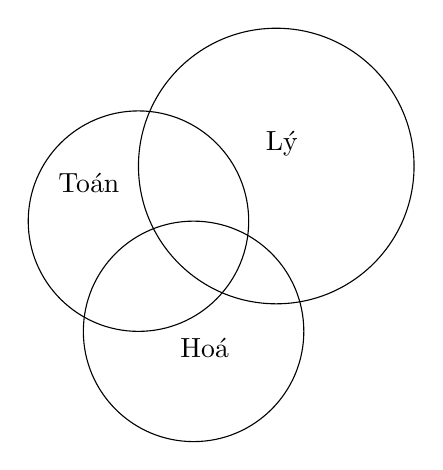
\begin{tikzpicture}[scale=.7]
		 \draw (0,0) circle (2);
		 \draw (2.5,1) circle (2.5);
		\draw (1,-2) circle  (2);
		\node  at (-0.9,0.7) {\text{Toán}};
		\node at (2.6,1.4)  {\text{Lý}};
		\node  at (1.2,-2.3) {\text{Hoá}};
	\end{tikzpicture}
		 }
	} 
\end{bt}

% nguồn: MaHoaNH_TraLoiNgan_Lop10
\begin{bt}%[0D1V3-5]%[ma:c2eeddc5]
	Lớp có học sinh trong  đó có em học sinh học giỏi môn Toán, em học sinh học giỏi môn Văn, em học sinh học giỏi môn Tiếng Anh. Đồng thời có em học sinh học giỏi cả môn Toán và môn Văn, em học sinh học sinh giỏi cả môn Văn và môn Tiếng Anh, em học sinh học giỏi cả môn Toán và môn Tiếng Anh, biết rằng mỗi học sinh trong lớp học giỏi ít nhất một trong ba môn Toán, Văn, Tiếng Anh. Hỏi lớp 10A có bao nhiêu bạn học giỏi cả ba môn Toán, Văn, Tiếng Anh?
	 \shortans{5}
	\loigiai{ 
		\begin{center}
			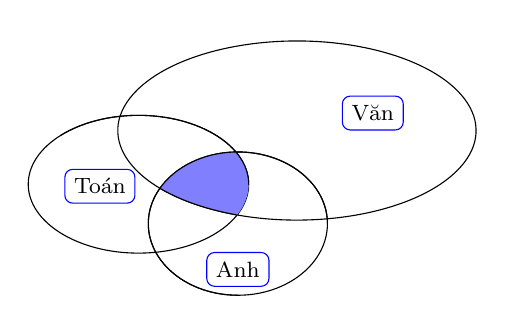
\begin{tikzpicture}[font=\footnotesize,line join=round,line cap=round,>=stealth]
					\tikzset{s/.style={draw=blue,rounded  corners=1mm,rectangle}}
					\def\a{3.5} 
					\def\b{0.55*\a} 
					\def\c{0.65*\a} 
					\def\e{0.5*\c} 
					 \def\f{0.5*\c}
					\def\g{0.4*\c} 
					\def\m{0.4*\a} 
					\def\n{0.25*\a} 
					 \fill[white,draw=black](60:{\a} and {\b}) arc (60:450:{\c} and {\e})
						(1,-0.5)  arc (0:360: {\f} and {\g})
						(0,0) arc  (0:360: {\m} and {\n});
					\begin{scope}
						\clip  (1,-0.5) arc (0:360: {\f} and {\g});
						 \clip (0,0) arc (0:360: {\m} and {\n});
						\fill[blue!50,draw=black](60:{\a} and {\b}) arc (60:450:{\c} and  {\e});
					\end{scope}
					 \draw
						(60:{\a} and {\b})++(80:-1) node[s,above]{Văn} 
						(0,0) arc (0:135: {\m} and {\n})++(120:-1) node[s,above]{Toán} 
						(1,-0.5) arc (0:270: {\f} and {\g})++(-90:-.55)  node[s,below]{Anh};
				\end{tikzpicture}
		\end{center}
		 Gọi $x$ ($x\in \mathbb{N}$) là số học sinh giỏi cả ba môn Toán, Văn, Anh.\\
		 Số học sinh chỉ giỏi Toán và Văn là $11-x$ (học sinh).\\
		Số học  sinh chỉ giỏi Toán và Anh là $9-x$ (học sinh).\\
		Số học sinh chỉ giỏi Văn và  Anh là $8-x$ (học sinh).\\
		Số học sinh chỉ giỏi Toán là $25-(11-x)-(9-x)-x$=5+x (học sinh).\\ 
		Số học sinh chỉ giỏi Văn là $23-(11-x)-(8-x)-x=4+x$ (học  sinh).\\
		Số học sinh chỉ giỏi Anh là $20-(9-x)-(8-x)-x=3+x$ (học  sinh).\\
		Lớp có $45$ học  sinh nên ta có
		 \[x+(11-x)+(9-x)+(8-x)+5+x+4+x+3+x=45\Leftrightarrow x+40=45\Leftrightarrow x=5. \]
		Vậy có $5$ học  sinh giỏi cả ba môn Toán, Văn và Anh.
	} 
\end{bt}


%%%%%%%%%%%%%%%% TỰ LUẬN %%%%%%%%%%%%%%%%

% nguồn: MaHoaNH_TuLuan_Lop10
\begin{bt}%[0D1H3-5]%[ma:f23bc3c7]
	Lớp $10$C có $45$ học sinh, trong đó có $18$ học sinh tham  gia cuộc thi vẽ đồ họa trên máy tính, $24$ học sinh tham gia cuộc thi tin học văn phòng cấp trường và $9$ học sinh không tham gia cả hai cuộc thi này. Hỏi có bao nhiêu học sinh của lớp $10$C tham gia đồng thời hai cuộc thi?
	\loigiai{ 
	Gọi $X$ là tập hợp các học sinh của lớp $10$C; $A$ là tập hợp các học sinh tham gia cuộc thi vẽ đồ họa trên máy tính và $B$ là tập hợp  các học sinh tham gia cuộc thi tin học văn phòng cấp trường.\\
	Theo giả thiết $n(A)=18$, $n(B)=24$,  $n(X)=45$.\\
	Do có $9$ học  sinh không tham gia cả hai cuộc thi nên số học sinh tham gia ít nhất một trong hai cuộc thi là
	 $$n(A\cup B) = 45 - 9 = 36.$$
	Suy ra số học sinh của lớp $10$C tham gia  đồng thời hai cuộc thi là
	$$n(AB) = n(A) + n(B) - n(A\cup B) = 18+24-36 =  6.$$
	} 
\end{bt}

% nguồn: MaHoaNH_TuLuan_Lop10
\begin{bt}%[0D1H3-5]%[ma:e040cc0d]
	 Trong số $35$ học sinh của lớp $10$H có $20$ học sinh thích môn Toán; $16$ học sinh thích môn Tiếng Anh và $12$ học sinh thích cả hai môn này.
	\begin{enumerate}
		\item Tính số học sinh thích ít nhất một trong hai  môn Toán và Tiếng Anh.
		\item Tính số học sinh không thích cả môn Toán và Tiếng Anh. 
	\end{enumerate}
	\loigiai{ 
	Gọi $A$, $B$ lần lượt là tập hợp các học sinh thích môn Toán và Tiếng Anh; $X$ là  tập hợp học sinh lớp $10$H.\\
	Theo giả thiết $n(A) = 20$, $n(B)=16$, $n(A\cap B) =  12$; $n(X) = 35$.
	\begin{enumerate}
		\item Số học sinh thích ít nhất một  trong hai môn Toán và Tiếng Anh là
		$$n(A\cup B) =  n(A)+n(B)-n(A\cup B) = 20+16-12=24.$$
		\item Số học sinh không thích cả môn Toán và Tiếng Anh  là
		 $$n(X)-n(A\cup B) = 35 - 24 = 11.$$
	\end{enumerate}
	} 
\end{bt}

% nguồn: MaHoaNH_TuLuan_Lop10
\begin{bt}%[0D1H3-5]%[ma:c756ac8c]
	Trong đợt văn nghệ chào  mừng ngày $20/11$, lớp $10 \mathrm{A}$ đăng kí tham gia hai tiết mục, đó là hát tốp ca và múa. Gọi $A$ là tập hợp các học sinh tham gia hát tốp ca, $B$ là tập hợp các học sinh tham gia múa, $E$ là tập hợp các học sinh của lớp. Mô tả các tập hợp sau đây:
	\begin{listEX}[2]
		\item  $A \cap B$.
		 \item $A \cup B$.
		\item $A \setminus  B$.
		 \item $E \setminus A$.
		\item $E \setminus(A \cup B)$. 
	\end{listEX}
	 \loigiai{
		\begin{listEX}
			\item $A \cap B$ là tập hợp các học sinh tham gia cả hai tiết mục là hát tốp ca và  múa.
			\item $A  \cup B$ là tập hợp các học sinh tham gia ít nhất một trong hai tiết mục là hát tốp ca hoặc múa.
			\item $A \setminus B$  là tập hợp các học sinh tham gia hát tốp ca nhưng không tham gia múa.
			\item $E \setminus A$ là tập hợp các học  sinh của lớp $10 \mathrm{A}$ không tham gia hát tốp ca.
			\item $E \setminus(A \cup B)$ là tập  hợp các học sinh của lớp $10 \mathrm{A}$ không tham gia tiết mục nào trong hai tiết mục hát tốp ca và múa.
		\end{listEX}
	} 
\end{bt}

% nguồn: MaHoaNH_TuLuan_Lop10
\begin{bt}%[0D1H3-5]%[ma:a5e5cd5a]
	Lớp $10 \mathrm{A}$ có $27$ học sinh tham gia ít nhất một trong  hai câu lạc bộ bóng đá và cờ vua, trong đó có $19$ học sinh tham gia câu lạc bộ bóng đá, $15$ học sinh tham gia câu lạc bộ cờ vua.
	\begin{listEX}
		\item Có bao nhiêu học sinh tham gia câu lạc bộ bóng đá mà  không tham gia câu lạc bộ cờ vua?
		\item Có bao nhiêu học sinh tham gia cả hai  câu lạc bộ?
		\item Biết trong lớp có $8$ học sinh  không tham gia câu lạc bộ nào trong hai câu lạc bộ trên. Lớp $10 \mathrm{A}$ có bao nhiêu học sinh?
	\end{listEX}
	\loigiai{ 
		Gọi $A$ là tập hợp các học sinh tham gia câu lạc bộ bóng đá, $B$ là tập hợp các  học sinh tham gia câu lạc bộ cờ vua.\\
		Khi đó $A \cup B$ là tập hợp các học sinh tham gia ít nhất một trong hai câu lạc  bộ bóng đá và cờ vua. Ta có số phần tử của $A$ là $19$, số phần tử của $B$ là $15$, số phần tử của $A \cup B$ là $27$.
		\begin{listEX}
			\item Tập hợp các học sinh tham gia câu lạc bộ  bóng đá mà không tham gia câu lạc bộ cờ vua chính là $A \setminus B$ và cũng là tập hợp $(A \cup B) \setminus B$.\\
			Số phần tử của tập hợp $(A \cup B) \setminus B$ chính là số phần tử của $A \cup B$ trừ đi  số phần tử của $B$.\\
			Vậy số học sinh tham  gia câu lạc bộ bóng đá mà không tham gia câu lạc bộ cờ vua là $27-15=12$ (học sinh).
			\item Tập hợp các học sinh tham gia cả hai  câu lạc bộ chính là tập hợp $A \cap B$.\\
			Số phần tử của $A \cap B$ bằng số phần tử  của tập hợp $A$ trừ đi số phần tử của tập hợp các học sinh chỉ tham gia câu lạc bộ bóng đá mà không tham gia câu lạc bộ cờ vua.\\
			Số học sinh tham gia cả hai câu  lạc bộ là $19-12=7$ (học sinh).
			\item Số học sinh của lớp $10 \mathrm{A}$ là $27+8=35$ (học  sinh).
		\end{listEX}
	 }
\end{bt}

% nguồn: MaHoaNH_TuLuan_Lop10
\begin{bt}%[0D1H3-5]%[ma:07406b06]
	Giải Bóng đá vô địch thế giới World Cup $2018$ được tổ chức ở Liên bang Nga gồm $32$ đội. Sau vòng thi đấu bảng, Ban tổ chức chọn ra $16$ đội chia  làm $8$ cặp đấu loại trực tiếp. Sau vòng đấu loại trực tiếp đó, Ban tổ chức tiếp tục chọn ra $8$ đội chia làm $4$ cặp đấu loại trực tiếp ở vòng tứ kết. Gọi $A$ là tập hợp $32$ đội tham gia World Cup $2018$, $B$ là tập hợp $16$ đội sau vòng thi đấu bảng, $C$ là tập hợp $8$ đội thi đấu vòng tứ kết.
	\begin{enumerate}
		\item Sắp xếp các tập hợp  $A, B, C$ theo quan hệ $\subset$.
		\item So sánh hai tập  hợp $A \cap C$ và $B \cap C$.
		\item Tập hợp $A\setminus B$ gồm những đội bóng bị loại  sau vòng đấu nào?
	\end{enumerate}
	\loigiai{\begin{enumerate}
	\item Ta có $A$ là tập  hợp $32$ đội tham gia World Cup $2018$.\\
	$B$ là  tập hợp $16$ đội sau vòng thi đấu bảng (chọn từ $32$ đội của tập hợp $A$ sau thi thi đấu theo bảng)\\
	Rõ ràng mỗi phần tử (mỗi đội) của tập hợp $B$ cũng là một phần tử  (một đội) của tập hợp $A$. Do đó $B \subset A$\\
	Từ $16$ đội của $B$, sau khi  đấu loại trực tiếp, còn lại $8$ đội vào tứ kết kí hiệu là tập hợp $C$. Do đó $C \subset B$.\\
	Vậy nên $C \subset B \subset A$. 
	\item Tập hợp $A \cap C$ gồm các đội bóng vừa thuộc $32$ đội tham gia World Cup $2018$,  vừa thuộc $8$ đội thi đấu vòng tứ kết, chính là $8$ đội của tập hợp $C$.\\
	Tập hợp $B \cap  C$ gồm các đội bóng vừa thuộc $16$ đội sau vòng thi đấu bảng, vừa thuộc $8$ đội thi đấu vòng tứ kết, chính là $8$ đội của tập hợp $C$.\\
	Vậy $A \cap C = B \cap C = C$. 
	\item Tập hợp $A\setminus B$ gồm  các đội thuộc $32$ đội tham gia World Cup $2018$ nhưng không thuộc $16$ đội sau vòng thi đấu bảng.\\
	Vậy  đó là $16$ đội không vượt qua vòng thi đấu bảng.\\
	Nói cách khác tập hợp $A\setminus B$ gồm các đội bóng bị loại sau vòng  đấu bảng.
\end{enumerate}
 }
\end{bt}

% nguồn: MaHoaNH_TuLuan_Lop10
\begin{bt}%[0D1H3-5]%[ma:d84acd97]
	Một cuộc khảo sát về khách du lịch thăm vịnh Hạ Long cho thấy trong $1\,410$ khách du lịch được phỏng vấn có $789$ khách du lịch đến thăm động Thiên Cung, $690$ khách du lịch đến đảo Titop. Toàn bộ khách được phỏng vấn đã đến ít nhất một trong hai địa điểm trên. Hỏi có bao nhiêu khách du lịch vừa đến thăm động Thiên Cung vừa  đến thăm đảo Titop ở vịnh Hạ Long?
	\loigiai{ 
	 \immini
	 {
	Gọi $A$ là tập hợp các khách du lịch đến thăm động Thiên Cung; $B$ là tập hợp các  khách du lịch đến đảo Titop. \\
	Suy ra $n(A)  = 789$; $n(B) = 690$; $n(A\cup B)=1\,410$.\\
	Biểu  đồ Ven như hình vẽ.
	 }
	 {
	\begin{tikzpicture}[scale=0.8,>=stealth,font=\footnotesize,line join=round,line cap=round]
			\draw (-1,0) ellipse (1.8 and 1.2); 
			\node at (-1.7,0)  {$A$};
			\draw (1,0) ellipse (1.8 and  1.2);
			 \node at (1.7,0) {$B$};
			\begin{scope}
				\clip (-1,0) ellipse (1.8  and 1.2);
				\fill[pattern=horizontal lines] (1,0) ellipse (1.8 and 1.2); 
			\end{scope}
		\end{tikzpicture}
	}\noindent 
	Tổng số khách du lịch bằng số khách đến động  Thiên Cung và số khách đến đảo Titop trừ đi số khách du lịch đến cả hai địa điểm.\\
	Khi đó $n(A \cup B) = n(A) + n(B) - n(A \cap B) \Leftrightarrow 1410 = 789 +  690 - n(A \cap B)\Leftrightarrow n(A \cap B)=69$.\\
	Vậy có $69$ khách du lịch vừa đến thăm động Thiên cung vừa đến thăm đảo Titop ở vịnh Hạ Long. 
	 }
\end{bt}

% nguồn: MaHoaNH_TuLuan_Lop10
\begin{bt}%[0D1H3-5]%[ma:c0e52ec1]
	 Một nhóm có $12$ học sinh chuẩn bị cho hội diễn văn nghệ. Trong danh sách đăng kí tham gia tiết mục múa và tiết mục hát của nhóm đó, có $5$ học sinh tham gia tiết mục múa, $3$ học sinh tham gia cả hai tiết mục. Hỏi có bao nhiêu học sinh trong nhóm tham gia tiết mục hát? Biết rằng có $4$ học sinh của nhóm không tham gia tiết mục nào.
	\loigiai{ 
		Kí hiệu $A$ là tập hợp học sinh tham gia tiết mục múa, $B$ là tập hợp  học sinh tham gia tiết mục hát, $E$ là tập hợp nhóm học sinh.\\
		Ta có thể biểu diễn ba tập hợp đó bằng biểu đồ  Ven như hình vẽ dưới đây.
		\begin{center}
			\begin{tikzpicture}[scale=1,font=\footnotesize,line join=round,line cap=round,>=stealth]
					\coordinate (A) at (0,0); 
					\coordinate (B) at  (2,0);
					\begin{scope}
						\clip[rotate=45] (A) ellipse (2cm and 1cm); 
						\fill[rotate=40,pattern=north west lines] (B) ellipse (2.2cm and  1.2cm);
					\end{scope}
					\draw[rotate=45] (A) ellipse (2cm and 1cm); 
					\draw[rotate=40]  (B) ellipse (2.2cm and 1.2cm);
					\draw  (-2,-2) rectangle (4,2.3);
					\draw[->]  (-3,0)--(-2,0);
					\draw[->]  (-3,0)--(-2,0);
					\draw (-3,0)+  (180:.3) node{$E$};
					 \draw (0,1.5) node{$A$}
						(0,0) node{$2$}; 
					 \draw (2.5,1.85) node{$B$}
						 (1,0) node{$3$}
						(3,-1.5)  node{$4$};
				\end{tikzpicture}
		\end{center}
		Khi đó, $A\cap B$ là  tập hợp học sinh tham gia cả hai tiêt mục.\\
		Số phần  tử của tập hợp $A$ là $5$, số phần tử của tập hợp $A\cap B$ là $3$, số phần tử của tập hợp $E$ là $12$.
		Số học sinh tham gia ít nhất một trong hai tiết mục là $12-4=8$ (học  sinh).\\
		Số học sinh tham gia  tiết mục hát mà không tham gia tiết mục múa là $8-5=3$ (học sinh).\\
		Số học sinh tham gia tiết mục  hát là $3+3=6$ (học sinh).
	 }
\end{bt}

% nguồn: MaHoaNH_TuLuan_Lop10
\begin{bt}%[0D1H3-5]%[ma:361217c5]
	Để phục vụ cho một hội nghị quốc  tế, ban tổ chức huy động $35$ người phiên dịch tiếng Anh, $30$ người phiên dịch tiếng Pháp, trong đó có $16$ người phiên dịch được cả hai thứ tiếng Anh và Pháp. Hãy trả lời các câu hỏi sau
	\begin{enumerate}
		\item Ban  tổ chức đã huy động bao nhiêu người phiên dịch cho hội nghị đó?
		\item  Có bao nhiêu người chỉ phiên dịch được tiếng Anh?
		\item Có bao nhiêu người chỉ phiên dịch  được tiếng Pháp?
	\end{enumerate}
	 \loigiai{
	 \immini
	{ 
	 Gọi $A$ là tập hợp những người phiên dịch tiếng Anh, $B$ là tập hợp những người phiên dịch tiếng Pháp. \\
	Ta  có $n(A)=35$; $n(B)=30$. \\
	Biểu  đồ Ven như hình vẽ.
	 }
	{ 
	\begin{tikzpicture}[scale=0.8,>=stealth,font=\footnotesize,line join=round,line cap=round]
			\draw (-1,0) ellipse (1.8  and 1.2);
			\node at (-1.7,0)  {$A$};
			\draw  (1,0) ellipse (1.8 and 1.2);
			\node at (1.7,0)  {$B$};
			\begin{scope}
				\clip (-1,0) ellipse (1.8 and  1.2);
				 \fill[pattern=horizontal lines] (1,0) ellipse (1.8 and 1.2);
			\end{scope}
		\end{tikzpicture}
	} 
	\begin{enumerate}
		\item $n(A \cup B) =  n(A) + n(B) - n(A \cap B) = 35 + 30 - 16 = 49$.\\
		Vậy ban tổ chức đã huy động  $49$ người phiên dịch cho hội nghị đó.
		\item $n(A\setminus  B) = n(A) - n(A \cap B) = 35 - 16 = 19$.\\
		Vậy có $19$ người chỉ phiên dịch được tiếng Anh. 
		\item $n(B\setminus A) = n(B) - n(B \cap A) = 30 - 16 =  14$.\\
		Vậy có $14$ người chỉ phiên dịch được tiếng Pháp. 
	\end{enumerate}
	} 
\end{bt}

% nguồn: MaHoaNH_TuLuan_Lop10
\begin{bt}%[0D1H3-5]%[ma:06126473]
	Trong một cuộc khảo sát người tiêu dùng, trong $100$ người uống cà phê được khảo sát, có $55$ người thêm đường, $65$ người thêm sữa và $30$ người thêm cả đường và sữa. Trong số $100$ người  đó
	\begin{enumerate}
		\item Có  bao nhiêu người thêm ít nhất đường hoặc sữa?
		\item  Có bao nhiêu người không thêm đường hoặc sữa?
	\end{enumerate}
	\loigiai{ 
	\immini 
	{ 
	Kí hiệu $U$ là tập hợp $100$ người được khảo sát, $A$ là tập hợp  người thêm đường, $B$ là tập hợp người thêm sữa (trong số $100$ người đó).\\
	Khi đó tập $A \cap B$ là tập hợp người thêm cả đường và sữa và $A \cup B$ là  tập hợp người thêm ít nhất đường hoặc sữa.\\
	Sơ đồ Ven như  hình vẽ.
	 }
	 {
	\begin{tikzpicture}[scale=0.8,>=stealth,font=\footnotesize,line join=round,line cap=round]
			\draw (-3.5,-2)  rectangle (3.5,2);
			 \node at (-3.2,1.5) {$U$};
			\draw (-1,0) ellipse (1.8 and 1.2); 
			\node at  (-1.7,0) {$A$};
			\draw (1,0) ellipse (1.8  and 1.2);
			 \node at (1.7,0) {$B$};
			\begin{scope}
				\clip  (-1,0) ellipse (1.8 and 1.2);
				\fill[pattern=horizontal lines] (1,0) ellipse  (1.8 and 1.2);
			\end{scope}
			\draw[->] (0.1,-0.3) -- (0.1,-1.35) node[below] {$A \cap  B$};
		\end{tikzpicture}
	} 
	\noindent 
	Theo giả thiết ta có $n(A)=55$; $n(B)=65$; $n(A \cap  B)=30$.
	\begin{enumerate}
		\item Số  người thêm ít nhất đường hoặc sữa là
		$$n(A \cup B)=n(A)+n(B)-n(A \cap  B)=55+65-30=90.$$
		\item Số  người không thêm đường hoặc sữa là $n(U)-n(A \cup B)=100-90=10$.
	\end{enumerate}
	} 
\end{bt}

% nguồn: MaHoaNH_TuLuan_Lop10
\begin{bt}%[0D1H3-5]%[ma:02c92b04]
	Lớp 10B có $28$ học sinh tham gia câu lạc bộ thể thao và $19$ học sinh tham gia câu lạc bộ âm nhạ{Biết rằng có  $10$ học sinh tham gia cả hai câu lạc bộ trên}
	\begin{enumerate}
		\item Có bao nhiêu học sinh tham gia câu lạc bộ thể  thao và không tham gia câu lạc bộ âm nhạc?
		\item Có bao nhiêu học  sinh tham gia ít nhất một trong hai câu lạc bộ trên?
		\item Biết lớp 10B có  $40$ học sinh. Có bao nhiêu học sinh không tham gia câu lạc bộ thể thao? Có bao nhiêu học sinh không tham gia cả hai câu lạc bộ?
	\end{enumerate}
	 \loigiai{
		Kí hiệu $A$ là tập hợp học sinh tham gia câu  lạc bộ thể thao, $B$ là tập hợp học sinh tham gia câu lạc bộ âm nhạc, $E$ là tập hợp học sinh của lớp 10B. Ta có thể biểu diễn ba tập hợp trên bằng biểu đồ Ven như hình dưới đây.
		\begin{center}
			\begin{tikzpicture}[scale=1,font=\footnotesize,line join=round,line cap=round,>=stealth]
					\coordinate (A) at (0,0); 
					\coordinate  (B) at (2,0);
					\begin{scope}
						\clip[rotate=45] (A) ellipse  (2cm and 1cm);
						\fill[rotate=40,pattern=north west lines] (B)  ellipse (2.2cm and 1.2cm);
					\end{scope}
					 \draw[rotate=45] (A) ellipse (2cm and 1cm);
					\draw[rotate=40] (B) ellipse  (2.2cm and 1.2cm);
					\draw  (-2,-2) rectangle (4,2.3);
					\draw[->]  (-3,0)--(-2,0);
					\draw[->] (-3,0)--(-2,0); 
					 \draw (-3,0)+ (180:.3) node{$E$};
					\draw (0,1.5) node{$A$} 
						 (0,0) node{$18$};
					\draw  (2.5,1.85) node{$B$}
						(2.5,0) node{$9$} 
						 (1,0) node{$10$};
				\end{tikzpicture}
		\end{center}
		Khi đó, $A\cap B$ là tập hợp học sinh tham gia cả hai câu lạc bộ trên. Số  phần tử của $A$ là $28$, số phần tử của $B$ là $19$, số phần tử của tập hợp $A\cap B$ là $10$.
		\begin{enumerate}
			\item Tập hợp các học sinh tham gia câu lạc bộ thể thao và không tham gia câu lạc bộ âm nhạc là tập hợp $A\backslash B$. Số phần tử của $A\backslash B$ chính là số phần tử của $A$ trừ đi số phần tử của $A\cap B$. Vậy số học sinh tham gia câu lạc bộ thể  thao và không tham gia câu lạc bộ âm nhạc là $28-10=18$ (học sinh).
			\item Tập hợp các học sinh tham gia ít nhất một trong hai câu lạc bộ trên chính là tập hợp $A\cup B$. Do khi đếm số học sinh tham gia câu lạc bộ thể thao là $28$, số học sinh tham gia câu lạc bộ âm nhạc là $19$ thì số học sinh tham gia cả hai câu lạc  bộ là $10$ được tính hai lần. Vậy số học sinh tham gia ít nhất một trong hai câu lạc bộ trên là $28+19-10=37$ (học sinh).
			\item Số phần tử của $E$ là $40$. Tập hợp các học sinh không tham gia câu lạc bộ thể thao là phần bù của $A$ trong $E$. Vậy số học sinh không  tham gia câu lạc bộ thể thao là $40-28=12$ (học sinh).\\
			Tập hợp các học sinh không tham gia cả hai câu lạc bộ là phần bù của $A\cup B$ trong $E$. Vậy số học sinh không  tham gia cả hai câu lạc bộ là $40-37=3$ (học sinh).
		\end{enumerate}
	} 
\end{bt}

% nguồn: MaHoaNH_TuLuan_Lop10
\begin{bt}%[0D1V3-5]%[ma:dcf39b05]
	Hai bạn An và Bình thường xuyên đến thư viện trường để đọc sách. Trong tháng $3$, số ngày An đến thư viện là $14$ ngày còn Bình đến thư viện $15$ ngày trong đó $10$ ngày cả  hai bạn cùng đến thư viện. Hỏi trong tháng $3$ đó có bao nhiêu ngày cả An và Bình đều không đến thư viện?
	\loigiai{ 
		Gọi $A$, $B$ lần lượt là tập hợp các  ngày An, Bình đến thư viện. Khi đó, $A\cap B$ là tập hợp các ngày cả hai bạn cùng đến thư viện, $A\cup B$ là tập hợp các ngày hoặc An đến thư viện hoặc Bình đến thư viện.\\
		Ta có $n(A)=14$, $n(B)=15$, $n(A\cap B)=10$.\\ 
		Số ngày hoặc An đến thư viện hoặc Bình đến thư viện là\\ 
		$n(A\cup  B)=n(A)+n(B)-n(A\cap B)=14+15-10=19$ (ngày).\\
	Tháng $3$ có $31$ ngày nên số ngày cả An và Bình đều không đến thư viện trong tháng  $3$ đó là $31-19=12$ (ngày).}
\end{bt}

% nguồn: MaHoaNH_TuLuan_Lop10
\begin{bt}%[0D1V3-5]%[ma:9f661876]
	Kết quả thi học kì của một trường THPT có 48 học sinh giỏi môn Toán (A), 37 học sinh giỏi môn Vật lí (B) và 42 học sinh giỏi môn Ngữ Văn (C). Biết rằng có 75 học sinh giỏi môn Toán hoặc môn Vật lí, 76 học sinh giỏi môn Toán hoặc môn Ngữ Văn, 66 học sinh giỏi môn Vật lí hoặc môn Ngữ Văn  và có 4 học sinh giỏi ba môn. Hỏi có bao nhiêu học sinh giỏi ít nhất 1 môn?
	 \loigiai{
		Ta có $n(A)=48, n(B)=37, n(C)=42$.  $n(A\cup B)=75, n(A\cup C)=76, n(B\cup C)=66$. $n(A\cap B\cap C)=4$.\\
		 Áp dụng công thức $n(A\cap B)=n(A)+n(B)-n(A\cup B)=48+37-75=10$.\\
		$n(A\cap  C)=n(A)+n(C)-n(A\cup C)=48+42-76=14$.\\
		$n(B\cap C)=n(B)+n(C)-n(B\cup  C)=37+42-66=13$.\\
		Số  học sinh giỏi ít nhất một môn là $n(A\cup B\cup C)$\\
		$n(A\cup B\cup C)=n(A)+n(B)+n(C)-n(A\cap B)-n(A\cap C)-n(B\cap C)+n(A\cap B\cap  C)$
		$n(A\cup B\cup C)=48+37+42-10-14-13+4=94$ (học  sinh).
	 }
\end{bt}

% nguồn: MaHoaNH_TuLuan_Lop10
\begin{bt}%[0D1V3-5]%[ma:9e1decb9]
	Đề thi học sinh giỏi trường môn Toán có $3$ câu tự luận. Sau khi chấm, giáo viên thống kê được như sau: Có $7$ học sinh làm được câu $1$, $5$ học sinh làm được câu $2$, $6$ học sinh làm được câu $3$, $3$ học sinh làm được cả câu $1$ và câu $2$, $4$ học sinh làm được câu $1$ và câu $3$, $2$ học sinh làm được câu $2$ và câu $3$, $1$ học sinh làm được cả $3$ câu. Hỏi có bao  nhiêu học sinh làm được ít nhất một câu?
	\loigiai{ 
		\begin{itemize}
			\item Số học sinh làm được câu $1$ và câu $2$ mà  không làm được câu $3$ là $3-1=2$.
			\item Số học sinh làm  được câu $1$ và câu $3$ mà không làm được câu $2$ là $4-1=3$.
			\item Số học sinh làm được câu $2$ và câu $3$ mà không làm được câu $1$ là $2-1=1$. 
			\item Số học sinh chỉ làm được  câu $2$ là $5-2-1-1=1$.
			\item Số học sinh  chỉ làm được câu $3$ là $6-3-1-1=1$.
			\item Số học sinh chỉ làm được  câu $1$ là $7-3-2-1=1$.
			\item Số học sinh làm ít nhất  một câu là số học sinh làm được $1$ câu hoặc $2$ câu hoặc cả $3$ câu $1+1+1+1+2+3+1=10$.
		\end{itemize}
	 }
\end{bt}

% nguồn: MaHoaNH_TuLuan_Lop10
\begin{bt}%[0D1V3-5]%[ma:18efe777]
	Một cửa hàng sách có ba loại sách khác nhau: sách văn học, sách khoa học và sách thiếu nhi. Hôm nay, cửa hàng đã bán được $20$ cuốn sách văn học, $15$ cuốn sách khoa học và $10$ cuốn sách thiếu nhi. Biết trong đó có $5$ cuốn sách vừa thuộc loại  văn học vừa thuộc loại khoa học, có $3$ cuốn sách vừa thuộc loại văn học vừa thuộc loại thiếu nhi, có $2$ cuốn sách vừa thuộc loại khoa học vừa thuộc loại thiếu nhi. Không có cuốn sách nào thuộc cả ba loại sách. Hãy tính tổng số cuốn sách khác nhau mà cửa hàng đã bán hôm nay.
	\loigiai{ 
		Ta có biểu đồ Ven như sau 
		\begin{center}
			\begin{tikzpicture}[smooth,font=\footnotesize,scale=0.8]
				\def\miena{(0,0) to[bend left=90] (3,3) to[bend left=90] (0,0)}
			\def\mienb{(3,3) to[bend left=90] (6,0) to[bend left=90] (3,3)}
			\def\mienc{(0.5,-0.5) to[bend left=90] (5.5,-0.5) to[bend left=90] (0.5,-0.5)}
			\draw \miena \mienb \mienc 
				 (4.7,0.2) node{$5$}
				(1.5,0.3)  node{$3$}
				 (3,2.2) node{$2$}
				(1,3.2)  node[rotate=40]{Thiếu nhi}
				(6,2.5) node[rotate=-45]{Khoa  học}
				(3,-2.3) node  {Văn}
				 (4.7,1.5) node{$15$}
				(1.5,1.3)  node{$10$}
				(3,-1) node{$20$}; 
			\end{tikzpicture}
		\end{center}
		Số cuốn sách chỉ thuộc thể  loại văn học: $20-3-5=12$.\\
		Số cuốn sách chỉ thuộc thể loại khoa  học: $15-5-2=8$.\\
		 Số cuốn sách chỉ thuộc thể loại thiếu nhi: $10-3-2=5$.\\
	Vậy,  tổng số cuốn sách khác nhau mà cửa hàng đã bán hôm nay là $12+8+5+3+5+2=35$ cuốn.}
\end{bt}
